\chapter{Decrease search range method}

\textbf{falta revisar seccion linear fit}

In the previous chapter we saw that the BGSEES algorithm for detecting the location of an EUV source (in this case, the Sun) is possible with a first, brute force approach. Here, the algorithm is studied in more detail considering a different method aiming to increase its precision and reduce its computational complexity.

\section{Decreasing the range of the search}

As we saw in the previous chapter, to increase the precision of the algorithm, the \textit{step} with which we iterate over the possible angles (right ascension and declination) is reduced. This causes more possible Suns to be considered. For example, with a step of one degree, we consider all possible right ascensions [0,360] and declinations [-90,90]: $360*180 = 64800$ Suns, minus the $2*360 - 2 = 718$ right ascensions we don't consider\footnote{We don't consider the 360 right ascensions of the two poles (-90 and 90), hence 2*360, but we do consider the two poles themselves (with any valid right ascension)} because as we have seen right ascensions for declinations of -90 and 90 are the same location.

We want to have the highest precision possible without having to consider all $64800 - 718 = 64082$ possibilities by progressively reducing the search range.

\section{Pseudocode}

This first optimization works as follows: the entire possible range is considered with a large starting step (e.g 60). Once the best Sun is found within this range, the precision is increased (the step is decreased) and the search range is reduced. This way the precision is increased but the number of considered possibilities remains similar each iteration of the algorithm. The following is the pseudocode\footnote{The code for the special cases of -90 and 90 degree declinations is not included for more readability. It is included in the implementation, in the following section.} for the algorithm using this optimization:

\begin{algorithm}
	\caption{Search range decrease}\label{searchRangeDecrease}
	\begin{algorithmic}[1]
		\Procedure{main}{}
		\State $\textit{epoch} \gets \text{findSpikeInData()}$
		\State $\text{filterDataByEpoch(\textit{epoch})}$
		\State $bestSun \gets nil$
		\State $r \gets \text{defaultRange()}$
		\For {$step = initStep; step >= min; step\ /= 2$}
		\For {$ra = r.lowerRa;\ ra <= r.upperRa;\ ra += step$}
		\For {$dec = r.lowerDec;\ dec <= r.upperDec;\ dec += step$}
		\State $currentSun \gets computeCorrelationPossibleSun(ra, dec)$
		\If {$currentSun.correlation > bestSun.correlation$}
		\State $bestSun \gets currentSun$
		\State $r \gets \text{newRange(\textit{bestSun, step})}$
		\EndIf
		\EndFor
		\EndFor
		\EndFor
		\\
		\Return $bestSun$
		\EndProcedure
	\end{algorithmic}
\end{algorithm}

\section{Implementation}

This first piece of code is the main loop of the method, which starts with a default range of ra=[0, 360], dec=[-90, 90] and is reduced every iteration based on the current best Sun's estimated location.

Furthermore, because an increase in the precision of the tested location doesn't necessarily imply an improvement in the solution, the new candidate is inserted into a \textit{priorityQueue} ordered by the coefficient to assure that the method returns the best one found throughout the entire execution.

\begin{minipage}{\linewidth}
	\begin{lstlisting}[language=c, caption=Decreasing the range and increasing the precision]
void TraverseGlobe::decreasingSTEP() {
	int rangeSize = 3;
	int initStep = 60;
	possibleSunInfo currentSun;
	searchRange range = setRange(currentSun, true, initStep, rangeSize);
	for (double step = initialStep; step >= 0.5; step /= 2) {
		currentSun = considerPossibleSuns(step, range, plotData);
		bestSuns.push(currentSun);
		range = setRange(currentSun, false, step, rangeSize);
	}
}\end{lstlisting}
\end{minipage}

The \textit{setRange} function sets a new range based on the estimated location that depends on the precision used for the values and checks that valid range values are returned.

\begin{minipage}{\linewidth}
	\begin{lstlisting}[language=c, caption=Setting the new range based on the estimated source location]
searchRange setRange(possibleSunInfo sun, bool defaultR, double step, int rangeSize) {
	searchRange range;
	if (defaultR) {
		range.lowerRa = 0;
		range.upperRa = 360;
		range.lowerDec = -90;
		range.upperDec = 90;
	}
	else {
		double raRange = step*rangeSize;
		double decRange = step*rangeSize;
		range.lowerRa = sun.ra - raRange >= 0 ? sun.ra - raRange : 0;
		range.upperRa = sun.ra + raRange <= 360 ? sun.ra + raRange : 360;
		range.lowerDec = sun.dec - decRange >= -90 ? sun.dec - decRange : -90;
		range.upperDec = sun.dec + decRange <= 90 ? sun.dec + decRange : 90;
	}
	return range;
}\end{lstlisting}
\end{minipage}

Finally, the \textit{considerPossibleSuns} function has the same functionality as the one from the previous chapter, it iterates over the possible locations, this time, however, it does so over the given range, rather than just the default one.

The names of the lower and upper bound variables have been changed (\textit{uRa} instead of \textit{upperRa}, for example) for readability.

\begin{minipage}{\linewidth}
	\begin{lstlisting}[style=myCStyle, caption=Iterating over possible locations within the given range]
possibleSunInfo considerPossibleSuns(double step, searchRange range) {
	FortranController fc;
	double pearsonCoefficient;
	int i = 0;
	possibleSunInfo bestSun;
	bestSun.coefficient = -23;
	bestSun.location = "salu2";

	for (double dec = range.lDec; dec <= range.uDec; dec += step) {
		if (dec != -90 and dec != 90) {
			for (double ra = range.lRa; ra <= range.uRa; ra += step) {
				pearsonCoefficient = fc.computeCorrelation(&ra, &dec);
				if (pearsonCoefficient > bestSun.coefficient) {
					bestSun.coefficient = pearsonCoefficient;
					bestSun.ra = ra;
					bestSun.dec = dec;
				}
			}
		}
		else {
			//Do only once
			double ra = 0;
			pearsonCoefficient = fc.computeCorrelation(&ra, &dec);
			if (pearsonCoefficient > bestSun.coefficient) {
				bestSun.coefficient = pearsonCoefficient;
				bestSun.ra = ra;
				bestSun.dec = dec;
			}
		}
	}
	return bestSun;
}\end{lstlisting}
\end{minipage}

Finally, the \textit{computeCorrelation} calls the Fortran code (the same used in the Brute Force chapter) to compute the correlation

Figure \ref{fig:consideredSolutions} is a visual representation of how the algorithm works. The X and Z axis are the possible right ascensions
and declinations (the possible solutions to our problem) and the Y axis is the correlation coefficient.

\begin{figure}[!htb]
	\begin{centering}
		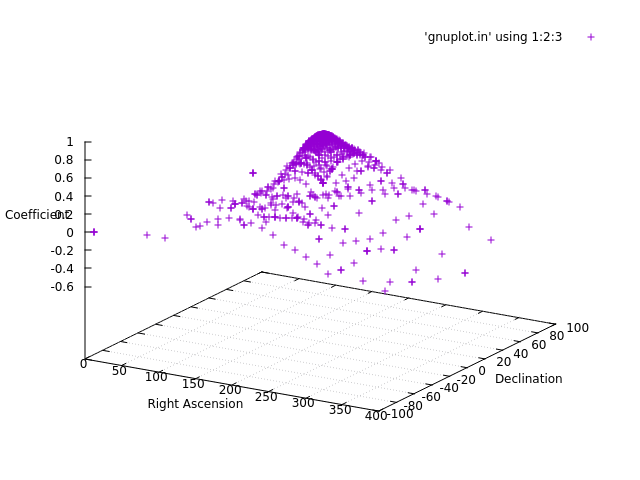
\includegraphics[width=0.5\linewidth]{images/ch6/hillClimbing/resultsAll.png}
		\caption{All visited candidates of the solution space}
		\label{fig:consideredSolutions}
	\end{centering}
\end{figure}

As we can see in the plot, as we increase the precision of the search, the range decreases, this can be seen because each point
of the plot is each of the locations considered by the algorithm: the density of considered solutions increases as the algorithm gets closer to the local maxima, the correct solution we are looking for.

Another change that could be done to improve this method's performance would be to adopt a sort of \textit{"Dynamic Programming"} strategy in order to avoid repeated calculations (the new range will always be inside the previous range). However, the problem is that because we are dealing with a different precision for the right ascension and declination values every loop, the same values are never used.

\section{Linear fitting: discarding outliers}

TODO: REVISAR ESTA SECCION

In the previous chapter we used a simple method to discard outliers for the VTEC value (using a cutoff value between -0.3 and 0.3). While this worked with that case in particular, using it with other data sets can lead to problems.

Because of this, another approach is presented in order to discard outliers: linear fitting. The aim is to find the line that fits best the relation between both variables (cosine and VTEC) by means of linear regression to discard samples that do not fit in it.

We can see that this procedure has been used before in figure \ref{fig:halloweenPaper} from the paper \textit{"GNSS measurement of EUV photons flux rate during strong and mid solar flares"}\cite{hernandez2012gnss}.

Manuel Herández-Pajares, the author, provided the Fortran program that performs this computation. After integrating it with the rest of the code, figure \ref{fig:linearFit} shows the result of testing it with the flare used in the previous chapter:

\begin{figure}[!htb]
	\begin{centering}
	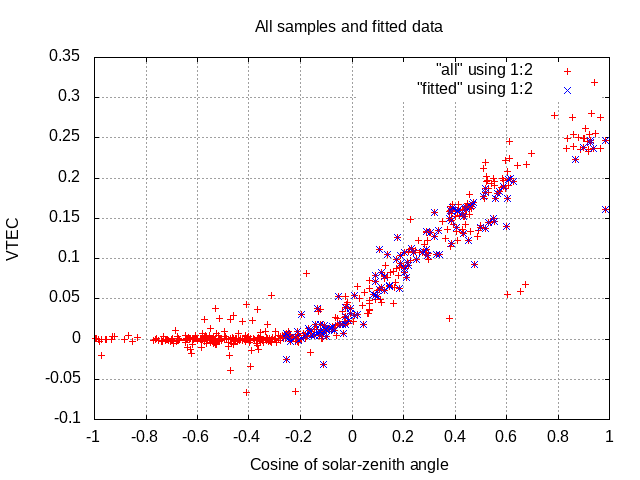
\includegraphics[width=0.5\linewidth]{images/ch6/linearFit/resultAll.png}
		\caption{All data (red) and fitted samples (blue)}
		\label{fig:linearFit}
	\end{centering}
\end{figure}

The main problem of this method is that before the correlation could be calculated in a single pass of the data. Now, on the other hand, the algorithm needs multiple iterations: first, the solar-zenith angle cosine for each IPP is calculated; then, the outliers are discarded, and finally the filtered data is traversed one last time to compute the correlation.

Here is the new code in order to compute the correlation for each possible location:

\begin{minipage}{\linewidth}
\begin{lstlisting}[style=myCStyle, caption=Discarding outliers and computing the correlation]
double computeCorrelation(double* ra, double* dec) {
	FileManager fileManager;
	int sigma = 1;
	int iterations = 6;
	computecosinesofcurrentsourcefortran_(ra, dec);
	fileManager.discardOutliersLinearFitFortran(sigma, iterations);
	return computecorrelationfortran_(ra, dec);
}\end{lstlisting}
\end{minipage}

As we can see, the data is traversed \textbf{at least} 3 times now (more depending on the number of iterations).

\section{Results}

Comparacion sencilla entre outliers/no-outliers, decir que en results mas detalle con otros ejemplos

Seeing the increase in computational complexity of this method because of the fact that outliers have to be discarded using the linear fitting method, we decided to instead focus on a different method that would rely only on the data itself, instead of considering the many possible locations of the source.
